\def\sectionName{罗峰为什么是神}
\section[\TOCName]{\sectionName}



\begin{frame}

% 如果它是 beamer
\if 1\isBeamerMode\relax
    {\Huge \sectionName}\par
\fi

% %%%%%%%%%%%%%%%%%%%%%%%%%%%%%%%%%%%%%%%%%%%%%%%%%%%%%%%%%%%%%%%%%%%%%%%%%%%%%
% 在这里填入你的名字
% %%%%%%%%%%%%%%%%%%%%%%%%%%%%%%%%%%%%%%%%%%%%%%%%%%%%%%%%%%%%%%%%%%%%%%%%%%%%%
\sectionAuthor{Ryeblablabla}{Ryeblablabla}



% %%%%%%%%%%%%%%%%%%%%%%%%%%%%%%%%%%%%%%%%%%%%%%%%%%%%%%%%%%%%%%%%%%%%%%%%%%%%%
% 这里可以写感想(嘲讽,bushi),也可以不写!!!
% %%%%%%%%%%%%%%%%%%%%%%%%%%%%%%%%%%%%%%%%%%%%%%%%%%%%%%%%%%%%%%%%%%%%%%%%%%%%%
罗峰为什么是神?在讨论这个问题之前,我们先说说其他选手相较于罗峰究竟差在了哪里?

\begin{center}
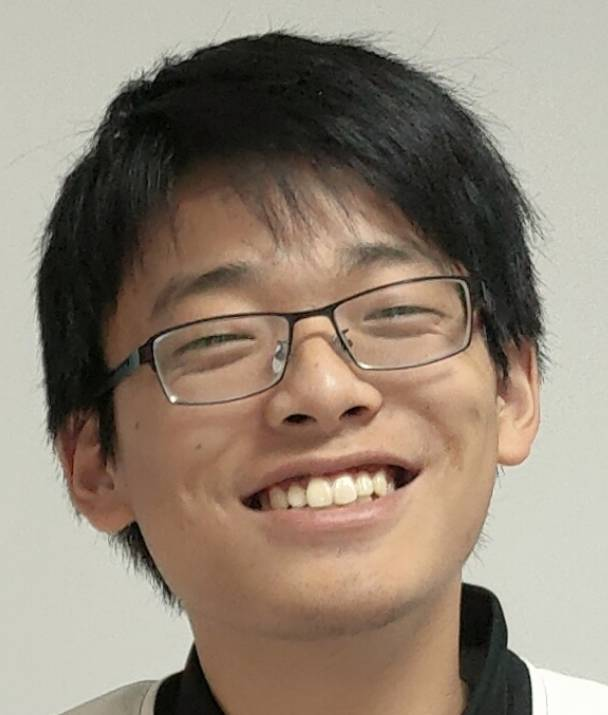
\includegraphics[width=0.3\textwidth]{./pic/luofeng.jpg}
\end{center}

\end{frame}

% %%%%%%%%%%%%%%%%%%%%%%%%%%%%%%%%%%%%%%%%%%%%%%%%%%%%%%%%%%%%%%%%%%%%%%%%%%%%%
% 这里开始写简单的题目意思 ~
% %%%%%%%%%%%%%%%%%%%%%%%%%%%%%%%%%%%%%%%%%%%%%%%%%%%%%%%%%%%%%%%%%%%%%%%%%%%%%
\subsection{题目意思}
\begin{frame} % 如果一个 frame 写不下的话,多开几个就好了~
懂的都懂。
\end{frame}



% %%%%%%%%%%%%%%%%%%%%%%%%%%%%%%%%%%%%%%%%%%%%%%%%%%%%%%%%%%%%%%%%%%%%%%%%%%%%%
% 这里开始写题解 ~
% %%%%%%%%%%%%%%%%%%%%%%%%%%%%%%%%%%%%%%%%%%%%%%%%%%%%%%%%%%%%%%%%%%%%%%%%%%%%%
\subsection{题解}
\begin{frame}
懂的都懂。
\end{frame}

